
\ExecuteOptions{letterpaper,oneside,12pt,onecolumn,final,openany}
\documentclass[12pt]{drexelthesis}
\usepackage{amsmath}
\usepackage{graphicx}
\usepackage{listings}
\graphicspath{{images/}}

\title{Automated Conversion of 3D Point Clouds to FEA Compatible Meshes}
\author{Matthew S.~Brown}
\advisor{Antonios~Kontsos, Ph.~D.~}


\begin{document}
\maketitle
\begin{preliminary}

%%%%%%%%%%%%%%%%%%%%%%%%%%%%%%%%%%%%%%%%%%%%%%%%%%%%%%%%%%%%%%%%%%%%%%%%%%%%%%%
\newpage
%%%%%%%%%%%%%%%%%%%%%%%%%%%%%%%%%%%%%%%%%%%%%%%%%%%%%%%%%%%%%%%%%%%%%%%%%%%%%%%

\setcounter{page}{2}

\date{} % Purposely left blank

%%%%%%%%%%%%%%%%%%%%%%%%%%%%%%%%%%%%%%%%%%%%%%%%%%%%%%%%%%%%%%%%%%%%%%%%%%%%%%%
\begin{dedication}

\end{dedication}
%%%%%%%%%%%%%%%%%%%%%%%%%%%%%%%%%%%%%%%%%%%%%%%%%%%%%%%%%%%%%%%%%%%%%%%%%%%%%%%

%%%%%%%%%%%%%%%%%%%%%%%%%%%%%%%%%%%%%%%%%%%%%%%%%%%%%%%%%%%%%%%%%%%%%%%%%%%%%%%
\begin{acknowledgements}

\end{acknowledgements}
%%%%%%%%%%%%%%%%%%%%%%%%%%%%%%%%%%%%%%%%%%%%%%%%%%%%%%%%%%%%%%%%%%%%%%%%%%%%%%%


%%%%%%%%%%%%%%%%%%%%%%%%%%%%%%%%%%%%%%%%%%%%%%%%%%%%%%%%%%%%%%%%%%%%%%%%%%%%%%%
\mytableofcontents\newpage

\addcontentsline{toc}{chapter}{List of Tables}
\setlength{\baselineskip}{0.5\baselineskip}
\listoftables\newpage

\addcontentsline{toc}{chapter}{List of Figures}
\listoffigures\newpage
\setlength{\baselineskip}{2.0\baselineskip}
%%%%%%%%%%%%%%%%%%%%%%%%%%%%%%%%%%%%%%%%%%%%%%%%%%%%%%%%%%%%%%%%%%%%%%%%%%%%%%%

%%%%%%%%%%%%%%%%%%%%%%%%%%%%%%%%%%%%%%%%%%%%%%%%%%%%%%%%%%%%%%%%%%%%%%%%%%%%%%%
\addcontentsline{toc}{chapter}{Abstract}
\begin{abstract}
This paper outlines a method to utilize machine learning in conjunction with advanced meshing techniques to autonomously segment raw point cloud data and reconstruct the resulting segments into simply connected volumetric meshes.

\end{abstract}

\clearpage
\end{preliminary}
\thispagestyle{empty}
\newpage
\

\setcounter{page}{0}
%%%%%%%%%%%%%%%%%%%%%%%%%%%%%%%%%%%%%%%%%%%%%%%%%%%%
% CHAPTER:                                                         INTRODUCTION
\chapter{Introduction}
\label{chap:introduction}

Surface reconstruction from a 3D point cloud is not a novel problem. In the past, groups have developed meshing algorithms for digital art replication, geographical topology analysis, and – more recently – structure health monitoring. All these processes, however, do not provide a general method to automate the entire pipeline between point-cloud collection and simple CAD geometry. We present a solution to this problem in the form of a robust and autonomous process for filtering, segmentation, and meshing of raw 3D point clouds.

%Related Works
\section{Related Work}
\label{sec:related}
[Introductory filler]
%%
\subsection{Geographical Topography Mapping}
\label{subsec:topographymapping}
In 2009, José Lerma and his team of archaeologists began using Terrestrial laser scanning in tandem with close proximity photogrammetry to render high resolution 3D surface models of ancient caves in Spain. Lerma et. al. are general in their description of their meshing method, which is most likely due to their non-computer programming oriented backgrounds. However, their pipeline involves sensor fusion between their laser scanner, which returns a pure point cloud with an origin at the center of the instrument, and deduced point clouds from photogrammetry data. The result is an impressive, high resolution surface mesh that accurately captures the features relevant to an archaeologist, but provide no useful information in terms of structural health monitoring %[1].
In 2014, Sebastian Siebert implemented similar technology mounted to UAVs to provide 3D mapping of earthwork projects for surveyors %[2].
%%
\subsection{Building Informational Modeling}
\label{subsec:BIM}
%[3]
%%
\subsection{Aerial Scanning for GPS Overlay
\label(subsec:UAVscanning}
%%
\subsection{Semi-Automated Point Cloud to FEA modeling}
\label{subsec:SemiFEA}
%[4] [5] [6] [7]
%
%
%%%%%%%%%%%%%%%%%%%%%%%%%%%%%%%
% Chapter: 		Background
\chapter{Background}
\label{chap:background}
%%
\section{Collection of Point Cloud Data}
\label{sec:PCcollection}
There are many ways of collecting point cloud data, ranging from implicit methods where the collection tool does not return direct xyz point data, such as stereogrammetry and structure from motion, to explicit methods where the direct return is a 3-dimensional position output, such as LiDAR, laser scanning and ultrasonic sensing. Each collection technique has its own set of parameters, accuracy ratings, and speed of collection / calculation.
\subsection{Implicit collection methods: Stereogrammetry and Structure from Motion}
\label{subsec:implicit}
[8]
\subsection{Explicit Methods: LiDAR, Laser Scanning, and Ultrasonic Sensing}
\label{subsec:explicit}
%%
\section{Sensor Fusion}
\label{sec:fusion}
%%
\section{Point Cloud Pre-processing Methods}
\label{sec:preprocessing}
\subsection{Registration}
\subsubsection{Position Data}
\subsubsection{Intrinsic Shape Signatures}
To stitch individual frames together, distinctive, repeatable features from each frame are found, and the most likely transformation between the frames is calculated via RANSAC estimation. There are numerous ways to classify distinctive features, but in this paper, we will focus on Intrinsic Shape Signatures due to its reliability and computational efficiency.
An intrinsic shape signature consists of two things:
\begin{itemize}
	\item An intrinsic reference frame
	\item A highly discriminative feature vector encoding the 3D shape characteristics
\end{itemize}
\subparagraph{Intrinsic Reference Frame Calculation}
\begin{enumerate}
	\item Compute a weight for each point $p_{i}$ inversely related to the number of points within 2-norm distance $r_{density}$:

		\begin{gather*}
		w_{i}=  \frac{1}{||p_{j} \mid |p_{j}-p_{i}| < r_{density}||}
		\end{gather*}
		This weight is used to compensate for uneven sampling of the 3D points, so that points at sparsely sampled regions contribute more than points at densely sampled regions. 

	\item Compute a weighted scatter matrix $cov(p_{i})$ for $p_{i}$ using all points $p_{j}$ within distance $r_{frame}$:
		\begin{gather*}
		cov(p_{i})= \sum{|p_{j}-p{i}| < r_{frame}}\frac{w_{j}(p_{j}-p_{i})(p_{j}-p{i})^{T}}{ \sum{|p_{j}-p{i}| < r_{frame}}w_{j}}
		\end{gather*}
	\item Compute the covariance matrix eigenvalues in order of decreasing magnitude and their resulting eigenvectors.
	\item $p_{i}$ is now the origin of the intrinsic frame, with $e^{1}$, $e^{2}$, and their cross product as the $x$, $y$, and $z$ axes, respectively [1].
\end{enumerate}

\subparagraph{3D Shape Feature Extraction}
The goal of the extraction is to create a view invariant “feature” vector providing us with some unique qualities about the point relationships within the intrinsic reference frame. At each point in the point cloud, or in increments of voxel stride size s, we build a sphere of some desired radius r centered at pi and divide it into 66 distinct partitions in angular space ($\theta, \psi$). A distinctive feature vector with 66 values is then computed by summing the radial distances ρi in each bin [1].

\begin{figure}
\centering
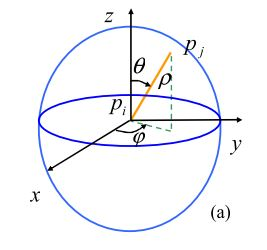
\includegraphics{ISSfeaturevector2.jpg}  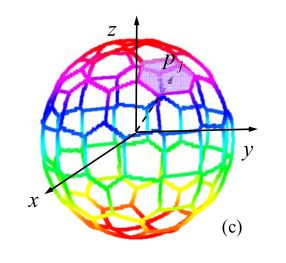
\includegraphics{ISSfeaturevector.jpg}
\caption[Intrinsic Shape Signature feature vectors]{Feature vector calculation via spherical bin decomposition [1]}
\end{figure}

\subsection{Flitering}
To minimize the amount of noise in the resulting dataset, a statistical approach requiring each point to have k neighbors within d standard deviations from the mean density radius of the cloud. This allows for controlled outlier removal, and a smoother cloud with fewer sharp edges.
\begin{gather*}
	P_{x} = p_{i} \mid \sum_{j=1}^n |p_{j} - p_{i}| \leq (r_{density} + d) \geq k
\end{gather*}

\begin{figure}
\centering
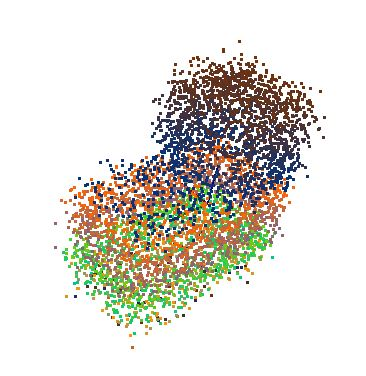
\includegraphics[width=2in]{l_block_pt_cloud10pnoise.jpg} 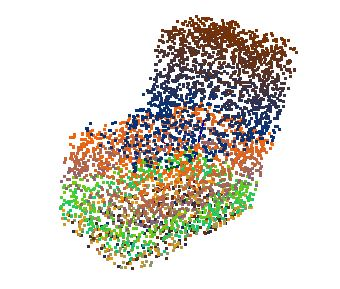
\includegraphics[width=2in]{l_block_pt_cloud10pnoiseFILTEREDk100std05.jpg}
\caption[Effects of noise filter on simulated point cloud objects]{The effects of noise filtering on a simulated L block with 10\% induced noise.}
\end{figure}


\subsection{Down-sampling}
Down-sampling is the process of fixing a point cloud’s mean density to a voxel of size n. This is done by iterating the voxel throughout the cloud’s entire volume and replacing all points occupying a voxel with a single point in the mean position of the voxel.

\begin{figure}
\centering
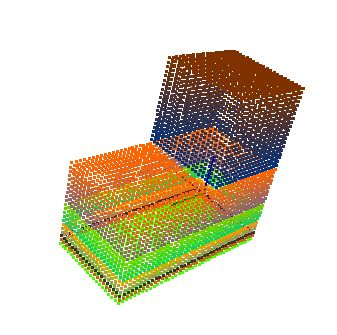
\includegraphics[width=2in]{l_block_pt_cloud} 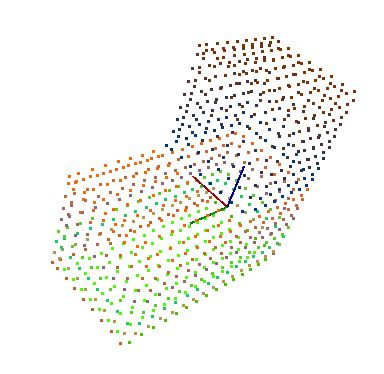
\includegraphics[width=2in]{l_block_pt_cloudDOWNSAMPLE025.jpg}
\caption[Effects of down-sampling on simulated point cloud objects]{A simulated L block point cloud down-sampled with voxel size = 0.25 $cm^{3}$.}
\end{figure}


\subsection{Dealing with Occlusion}
Occlusion is a common issue in the perception world, defined by the lack of information in an image / 3D scan due to other objects blocking a direct view. A simple example: In 3D scene reconstruction from images, it is impossible to accurately reconstruct the contents inside an opaque box because we cannot see inside the box. This is occlusion. In the field, it is nearly impossible to fully avoid occluded datasets when scanning an object via LiDAR equipped UAVs. It is crucial to be able to develop methods to alleviate this problem.

\begin{figure}
\centering
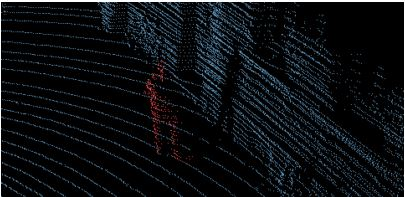
\includegraphics{occluded_man.jpg}
\caption[Demonstration of occlusion]{Section of a building occluded by an object in the foreground [11].}
\end{figure}


%%
\section{Machine Learning for Object Recognition and Segmentation}
\label{sec:machinelearning}
\subsection{Supervised Methods --- Neural Networks}
\subparagraph{Definitions}
It is difficult to define how a Convolutional Neural Network works without first defining a convolution. To detect distinctive features in a dataset – from a machine’s perspective – the dataset needs to be modified to enunciate those features. Key features in machine vision include edges, corners, and areas with distinctive geometry. Convolutions are the key to bringing these features to the forefront of the image.
A convolution kernel is a weighted square matrix of dimensions m, and depth equaling the rank of the feature space of the dataset. The kernel acts as a filter for the image as it strides from supervoxel to supervoxel. At each step, the dot product of the kernel with data values inside the current super-voxel provide a convolved image of the dataset while retaining characteristic features. The equation below illustrates the math behind a convolution kernel. C represents the convolved image, w the weight matrix, I the original image, m the size of the kernel, and i represents the voxel position.

[N DIMENSIONAL CONVOLUTION EQUATION]

Another type of convolution is called pooling, or subsampling. This convolution steps through the dataset with a stride value greater than one, resulting in a smaller image of the original set. In pooling, the kernel will pull either the largest intensity from each super-voxel, or the average intensity of the data points inside the super-voxel. This allows for the machine to decrease the size of the dataset while maintaining distinctive features.

\subparagraph{Convolutional Neural Networks}
Convolutional Neural Networks (CNNs) are modeled after the visual cortex in the brain. They consist of layers of convolutional networks. Each network contains “neurons” with simple feature reception fields. Through layers upon layers of these networks, objects can be classified. The biases and weights on these networks can be adjusted based on learning algorithms REF 1 in proposal. CNNs have become the standard in feature classification for image processing, but the accuracy that they provide comes at the price of processing time. 
Every CNN can be broken down into the following steps: Convolution, max/mean pooling, activation function, fully connected layer, repeat. The diagram below illustrates the overarching structure of a basic Convolutional Neural Network:
\begin{figure}
\centering
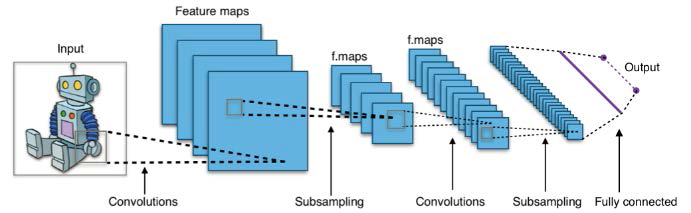
\includegraphics[width=6in]{cnn.png}
\caption[High level flow chart of a convolutional neural network]{Map of a convolutional neural network with two hidden layers [ref]}
\end{figure}

In the case of point cloud processing, the input is a raw xyz set of some size n x 3. The first step in the network is a series of convolutions of the dataset. Each kernel in the layer contains m x m x 3 trainable weights, which are iteratively modified using a steepest descent numerical solver during the training phase of the system. The convolved images are stacked in a block, called a feature map, or convolutional layer. From there, the convolved images are pooled (or subsampled) to condense the size of the image stack. 
At this point, there is a large stack of feature maps draw from the original input dataset. In a simple linear system, these features are combined into a single weighted summation function, where the input is each individual feature value, and the output is a vector representing the probability of the image belonging to a certain class.
\[
\begin{bmatrix}
C_{1} \\
\vdots \\
C_{n}
\end{bmatrix}  =  \begin{bmatrix} w_{1,1} & \hdots & w_{1,m+1} \\ \vdots & \ddots & \hdots \\ w_{n,1} & \hdots & w_{n, m+1} \end{bmatrix}  \begin{bmatrix} f_{1} \\ \vdots \\ f_{n} \\ 1 \end{bmatrix} \]

The equation above represents the transformation from feature space to the “fully connected layer.” $C_{i}$ represents the probability of the input image belonging to class $i$, and $f_{i}$ represents the value of the ith feature in the feature map. 
Linear classification methods limit the versatility of the CNN, as many object distinctions do not follow a linear pattern in $n$-dimensional space. To account for this, most CNNs – including the ones utilized in this paper – incorporate a de-linearizing element dubbed the “activation function.” The activation function applies a nonlinear operation to the values in the convolution layer, which allows for the CNN to become a very powerful nonlinear fit function. Typical activation functions include the hyperbolic tangent function, the sigmoid function, and – most popularly – the rectifier function. Each of these functions are show in the figure below:

\begin{figure}
\centering
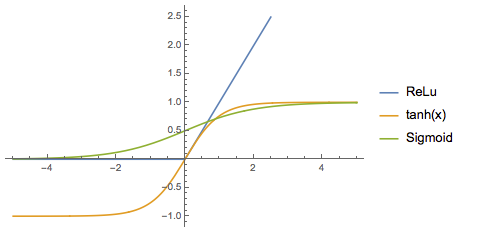
\includegraphics[width=5in]{cnnReLu.png}
\caption[Common CNN non-linear activation functions]{Visualization of commonly used non-linear activation functions}
\end{figure}

From input to output, all CNNs have the same skeleton structure, with a varying number of layers between the raw input and the fully connected layer:

\begin{figure}
\centering
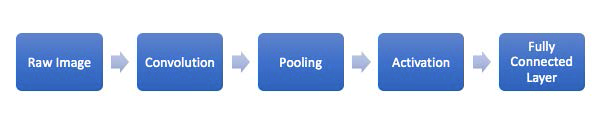
\includegraphics[width=6in]{cnn_flow.png}
\caption[Block diagram of CNN flow]{Block diagram of a CNN$'$s skeleton structure}
\end{figure}

For the system to be accurate, the weights for each convolution and connection must be trained. This training is done through a process called backpropagation. An image-set of known classifications is fed to the untrained system, and the error between the system’s classification and the true classification of each image is used to update the weights iteratively until the machine’s class prediction closely resembles ground truth. Most algorithms use numerical solving methods to sharply diminish the number of iterations required for convergence. The “gradient descent” method is commonly used in the machine learning world due to its rapid convergence properties and low computational complexity. The method is shown below:

\begin{gather*}
	x_{k+1} = x_{k} - \gamma \nabla F(x_{k})
\end{gather*}
 \[ F(x) =
\begin{bmatrix}
C_{1} \\
\vdots \\
C_{n}
\end{bmatrix}  -  \begin{bmatrix} w_{1,1} & \hdots & w_{1,m+1} \\ \vdots & \ddots & \hdots \\ w_{n,1} & \hdots & w_{n, m+1} \end{bmatrix}  \begin{bmatrix} f_{1} \\ \vdots \\ f_{n} \\ 1 \end{bmatrix} \]

The speed, accuracy, and versatility of a CNN are functions of the number of hidden layers, the size of the convolutional layers, the type of activation functions, and the size and versatility of the training dataset [12].

\subsection{Unsupervised Methods}
With our goal being to isolate specific objects in a structural health monitoring setting, the ideal segmentation method is a supervised learning algorithm, such as a convolutional neural network, that semantically parses the point cloud based on a training set of pre-defined cloud objects [9]. However, due to time limitations, and a lack of training data relevant to our objects of interest, this is not possible. Instead we explore a series of unsupervised clustering methods on the assumption that objects are distinct enough in relative cloud neighborhoods to be properly segmented.
\subparagraph{Methods Used}
\subsubsection{K-means Clustering}
K-means clustering is an iterative method that groups $n$-dimensional datasets into $k$ clusters based on a minimization of the Euclidean distance cost function $|x-c|^{2}$. Initially, $k$ centroids are placed randomly inside the dataset, and all data points are placed in bins $S$ depending on which centroid minimizes their cost function. At each iteration, the cluster centroids $c_{i}$ are re-calculated. Criteria for convergence is a maximum Euclidean distance change $σ$ between centroid position $c_{n}$ and $c_{n+1}$.
\begin{gather*}
	arg min_{S} \sum{i=1}^{k} \sum{x \in S_{i}} |x - c_{i}|^{2}
\end{gather*}

[PROS, CONS, AND GENERAL USAGE CASES]

\subsubsection{Fuzzy C-means Clustering}

Fuzzy C-means (FCM) is very similar to K-means clustering. Once again, points are iteratively grouped to k centroids based on their Euclidean distance to the centroid. The significant difference is that points do not belong exclusively to a single group. Instead, points are weighted by their degree of belonging in each cluster.

\begin{gather*}
	c_{k} = \frac{\sum{x}w_{k}(x)^{m}x}{\sum{x}w_{k}(x)^{m}}
\end{gather*}

Each point is provided a weight vector w [0, 1] for its likelihood of belonging in each cluster, where the weight function is as follows:

\begin{gather*}
	w_{ij} = \frac{1}{\sum_{k=1}^{c}(\frac{|x_{i}-c_{j}|}{|x_{i}-c_{k}|})^{\frac{2}{m-1}}}
\end{gather*}

[PROS, CONS, AND GENERAL USAGE CASES]

\subsubsection{Aggomerative and Dvisive Hierarchical Clustering}
In Agglomerative clustering, each point is initially considered its own cluster. Iteratively, the points are grouped together based on a user-defined cost function – in our case, Euclidean distance. The exit conditions for this method are either convergence upon a set of clusters, or a predefined number of clusters.
Divisive clustering approaches the clustering problem in an exactly opposite fashion. The algorithm initializes the dataset as a single cluster and iteratively splits the remaining clusters until reaching the same exit conditions as the Agglomerative method.


\begin{figure}
\centering
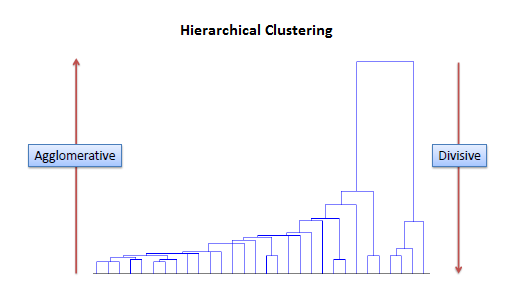
\includegraphics[width=4in]{divisiveAgglomerative.png}
\caption[Comparison of divisive and agglomerative clustering methods]{Comparison of divisive and agglomerative hierarchical clustering}
\end{figure}


\subsubsection{Euclidean Distance Clustering}
Perhaps the simplest of the algorithms listed above, Euclidean distance clustering operates on the pretense that objects are separated significantly enough spatially from another that clustering points based on their proximity to other points in the cloud is sufficient to properly segment the dataset. This algorithm involves no iterative process, and requires two inputs: Maximum point-to-point distance $r$, and minimum number of points per cluster $k$.

\subsubsection{Comparison of Methods}

 \begin{table}[h!]
     \begin{center}
           \caption[Comparison of Unsupervised clustering methods]{Comparision of unsupervised clustering methods on various simulated point clouds}
     \begin{tabular}{ | c | p{3cm} | p{3cm} | p{3cm} | p{3cm} | }
     \hline
      K-means & Fuzzy C-means & Agglomerative & Divisive & Euclidean \\ 
      \hline
      		\includegraphics[width=2cm]{2d-cluster-tests/k-means/concentric.jpg}
      & 
      		\includegraphics[trim={0 0 0 2cm},clip, width=2cm]{2d-cluster-tests/fcm/concentric.jpg}
      & 
      		\includegraphics[trim={0 1cm 0 1cm},clip, width=2cm]{2d-cluster-tests/agglomerative/concentric.jpg}
      &

      &
      		\includegraphics[width=2cm]{2d-cluster-tests/euclidean-distance/concentric.jpg}
      \\ \hline
      
            \includegraphics[width=1.5cm]{2d-cluster-tests/k-means/lines.jpg}
      & 
             \includegraphics[width=1.5cm]{2d-cluster-tests/fcm/lines.jpg}    
      & 
             \includegraphics[trim={0 1cm 0 0cm},clip,width=1.5cm]{2d-cluster-tests/agglomerative/lines.jpg}    
      &

      &
             \includegraphics[trim={0 1cm 0 1cm},clip, width=1.5cm]{2d-cluster-tests/euclidean-distance/lines.jpg}    
      \\ \hline
      
           \includegraphics[trim={0 1cm 0 1cm},clip,width=1.5cm]{2d-cluster-tests/k-means/blob.jpg}
      & 
           \includegraphics[trim={0 0cm 0 0cm},clip,width=1.5cm]{2d-cluster-tests/fcm/blob.jpg} 
      & 
           \includegraphics[trim={0 1cm 0 1cm},clip,width=1.5cm]{2d-cluster-tests/agglomerative/blob.jpg} 
      &

      &
           \includegraphics[trim={0 1cm 0 1cm},clip,width=1.5cm]{2d-cluster-tests/euclidean-distance/blob.jpg} 
      \\ \hline
      
            \includegraphics[trim={0 1cm 0 1cm},clip,width=1.5cm]{2d-cluster-tests/k-means/solid_circles.jpg}
      & 
            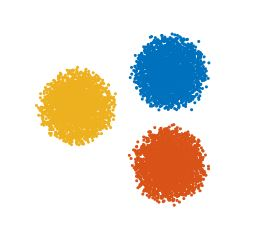
\includegraphics[trim={0 1cm 0 1cm},clip,width=1.5cm]{2d-cluster-tests/fcm/circles.jpg}
      & 
            \includegraphics[trim={0 1cm 0 1cm},clip,width=1.5cm]{2d-cluster-tests/agglomerative/solid_circles.jpg}
      &

      &
            \includegraphics[trim={0 1.5cm 0 1.5cm},clip,width=1.5cm]{2d-cluster-tests/euclidean-distance/solid_circles.jpg}
      \\ \hline
      
            \includegraphics[trim={0 1cm 0 1cm},clip,width=1.5cm]{2d-cluster-tests/k-means/plane.jpg}
      & 
            \includegraphics[trim={0 0cm 0 1cm},clip,width=1.5cm]{2d-cluster-tests/fcm/plane.jpg}
      & 
            \includegraphics[trim={0 1cm 0 1cm},clip,width=1.5cm]{2d-cluster-tests/agglomerative/plane.jpg}
      &
      
      &
            \includegraphics[trim={0 1cm 0 1cm},clip,width=1.5cm]{2d-cluster-tests/euclidean-distance/plane.jpg}
      \\ \hline
      
      \end{tabular}
      \end{center}
      \end{table}


\subsection{Converting a Discrete Point Cloud to a Bounded Area Surface Mesh} 
Surface meshing is the science of inferring a continuous shape topology from a discrete, $n$-dimensional point cloud. There are many different approaches to converting from discrete points to surface meshes, but at their core, nearly all of them rely on the Delaunay triangulation method.
Delaunay triangulation finds its routes in Voronoi tessellation, a method of constructing non-overlapping geometrical tiles. Voronoi tessellation states the following:
For a given set of points in space, $\{P_{k}\}$ --- $k$ = 1, \ldots, $K$, the regions \{$V_{k}$\} are polygons assigned to each seed point $P_{k}$, such that $V_{k}$ represents the space closer to $P_{k}$ than any other point in the set.

\begin{gather*}
	V_{k} = \{P_{i} \mid |p - P_{i}| < |p - P_{j}|, \forall j \neq i \}
\end{gather*}

If every point pair sharing a Voronoi boundary are connected, the result is a triangulation object encasing the pointset. This object is referred to as a Delaunay triangulation [13].

\begin{figure}
\centering
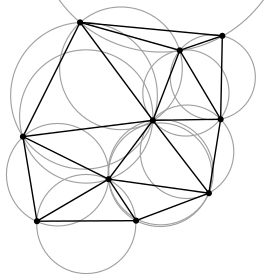
\includegraphics{delaunay.png}
\caption[2D delaunay triangulation]{Visual represention of a 2-dimensional delaunay triangulation process}
\end{figure}

\subsubsection{Advancing Front / Marching Triangles}
The Advancing Front method is common in computer graphics software – especially in procedurally generated games – because of it’s speed and computational simplicity.
[DEFINITION, USAGE, AND 2D EXAMPLE]
 [14]

\subsubsection{Scale Space Reconstruction Method}
At a grand scale, the Scale Space Reconstruction Method aims to optimize surface meshing in the face of discrete point cloud data. No matter how accurate or dense a point cloud may be, there is no way to verify the topology defined by the cloud is accurate to the true object topology. To simplify this ill-posed problem, and reduce mesh quality damage due to noisy points, the Scale Space algorithm casts the raw point cloud to a space of scale N by iteratively calculating the mean curvature of a neighborhood of points and casting each point pk to it’s nearest point on the curve. This results in a far more uniform point cloud, which can mesh via Delaunay triangulation at a high quality level. Once the meshing has occurred, the pointset is then recast to its original scale to maintain complex features. 

\textbf{Algorithm 1:} Mean Curvature Calculation

	\textbf{Input:} A point set $P$, a query point $p$, and a radius $r$.
	
	\textbf{Output:} A point $p'$, the result of one discrete step of the mean curvature calculation applied to $p$.
\begin{lstlisting}[escapeinside={(*}{*)}]
for ( (*$p$*) in (*$P$*) )
	get (*$neighbors$*) from (*$p$*)
	if num(neighbors) < 5
		remove (*$p$*)
	set (*$p_{bar} = \frac{\sum_{q \in neighbors} w(q)q}{\sum_{q \in neighbors}w(q)}$*)
	set (*$C = \sum_{q \in neighbors} w(q)(q-p_{bar})(q-p_{bar})^{2}$*)
	set (*$v_{0} = min eigenvector(C)$*)
	set (*$p' = p - \langle p - p_{bar}, v_{0} \rangle v_{0}$*)
	(*$p' \cdot n = \frac{p-p'}{|p-p'|} \cdot sign(\langle p - p', p \cdot n \rangle ) $*	
\end{lstlisting}

\textbf{Algorithm 2:} Scale Space Iterator

	\textbf{Input:} A point set $P$, a number of iterations $N$, and a radius $r$
	
	\textbf{Output:} A modified point set $P_{N}$


\begin{lstlisting}[escapeinside={(*}{*)}]
for (*$p$*) in (*$P$*)
	set (*$p.origin = p$*)
set idx = 0
for ( i = 0, \ldots, N-1 )
	new_idx = mod(idx, 2) + 1
	for (*$p \in P_{idx}$*)
		(*$p' = MCC(p, P_{idx}, r)$*)
		store (*$p'$*) in (*$ P_{new_idx}$*)
		(*$p'.origin = p.origin $*)
	if ( idx > 0 )
		remove (*$P_{idx}$*)
	idx = new_idx
\end{lstlisting}

\textbf{Algorithm 3:} Back Projection to Final Mesh

	\textbf{Input:} A point set $P$, a number of iterations $N$, and a radius $r$
	
	\textbf{Output:} A modified point set $P_{N}$


\begin{lstlisting}[escapeinside={(*}{*)}]
\end{lstlisting}

\begin{table}
\begin{centering}
\caption[Effect of increasing scale in a scale space reconstruction]{Effect of increasing scale in a scale space reconstruction}
\begin{tabular}{ | c | c | c | }
\hline
& 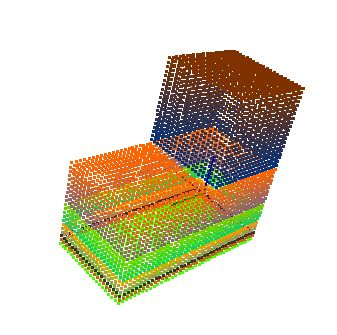
\includegraphics[width=3cm]{l_block_pt_cloud.jpg}
	Clean Point Cloud
& 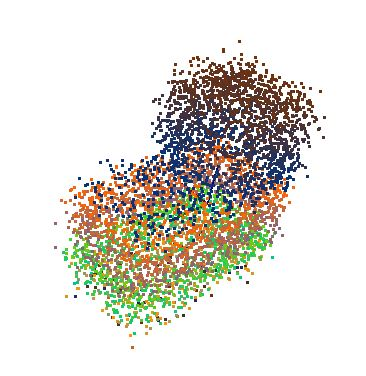
\includegraphics[width=3cm]{l_block_pt_cloud10pnoise.jpg}
	10\% Induced Noise
\\
\hline
Scale Space 3 & 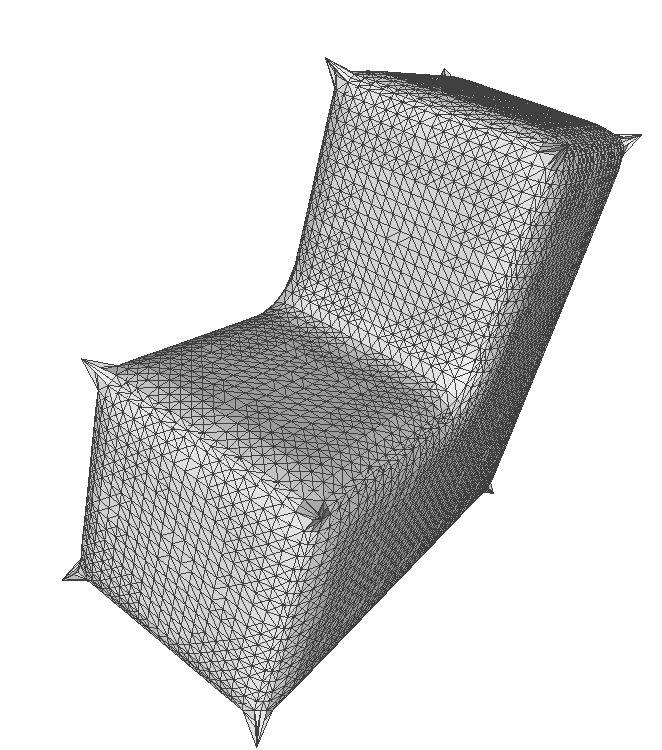
\includegraphics[width=3cm]{scalespace/clean/scalespace3.png} & 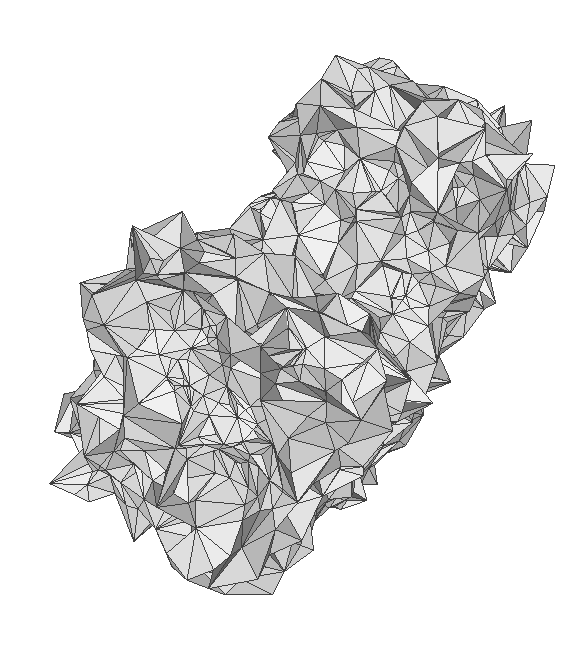
\includegraphics[width=3cm]{scalespace/10pnoise/scale3.png}
\\
\hline
Scale Space 5 & 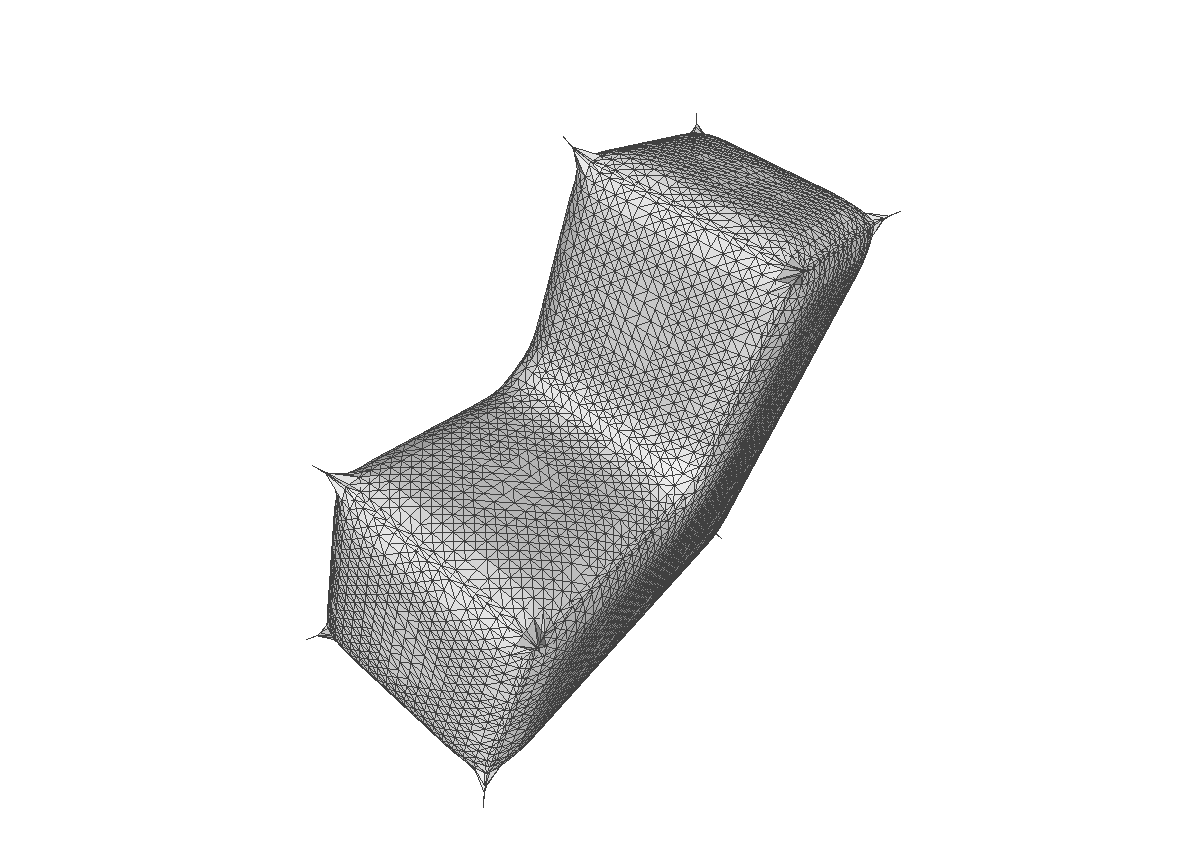
\includegraphics[width=3cm]{scalespace/clean/scalespace5.png} & 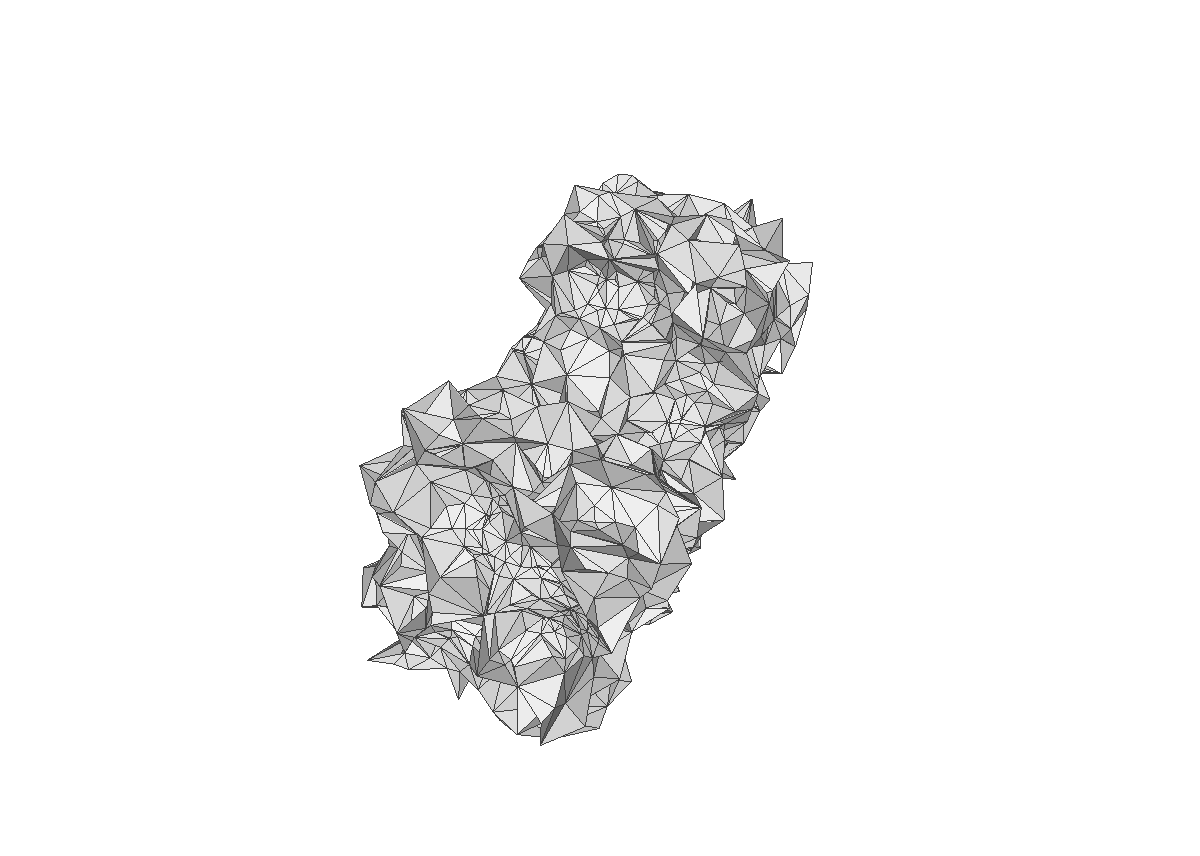
\includegraphics[width=3cm]{scalespace/10pnoise/scale5.png}
\\
\hline
Scale Space 10 & 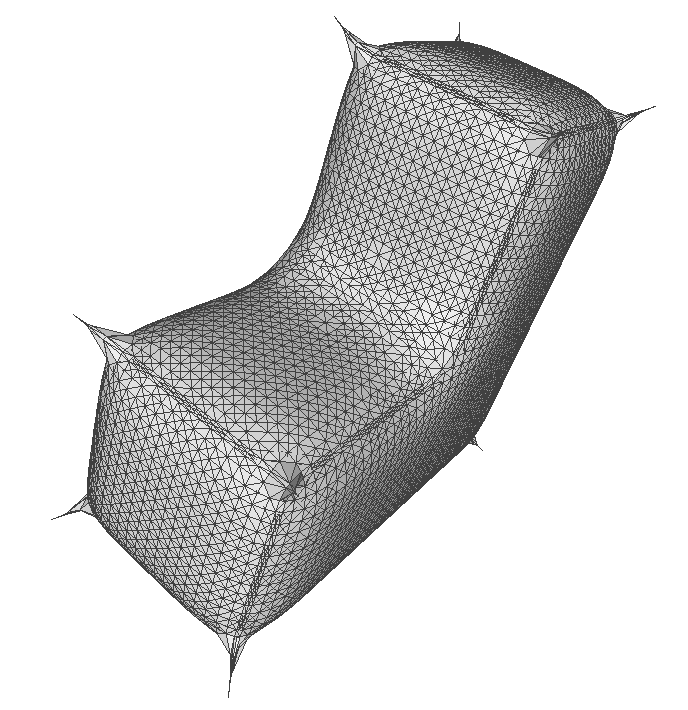
\includegraphics[width=3cm]{scalespace/clean/scalespace10.png} & 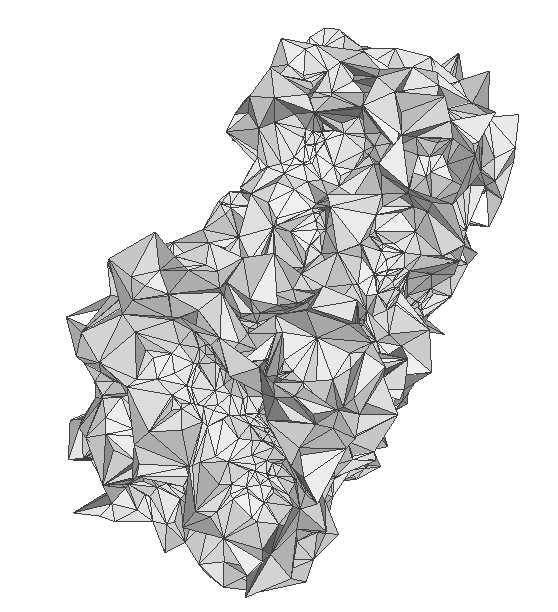
\includegraphics[width=3cm]{scalespace/10pnoise/scale10.png}
\\
\hline
\end{tabular}
\end{centering}
\end{table}


 

\subsubsection{Hole Patching, Fairing, and Refinement}

\subsection{Mesh Optimization}
Now that the objects in the cloud are properly segmented, they must be meshed in a way that is both accurate to the real-world definition of the object and suitable to be converted from a surface mesh to a volumetric mesh.

\subsubsection{Criteria for Mesh Quality and Failure Criteria for Volumetric Conversion}
Now that the objects in the cloud are properly segmented, they must be meshed in a way that is both accurate to the real-world definition of the object and suitable to be converted from a surface mesh to a volumetric mesh.

\subparagraph{Failure Criteria}
The first criterion for surface mesh compatibility with volumetric conversion is “water-tightness.” Meaning, there are no gaps, holes, or unbounded edges in the triangulation. These gaps can be quantified as any edge in a polyhedron that is referenced by no other polyhedron in the triangulation.
The other criteria are more abstract in nature and are more difficult to detect and handle independently. We define these criteria as mesh “Quality.” Quality is a quantification of the level of simplicity of a triangulation object by evaluating ratios of different elements in the triangulation.







%%%%%%%%%%%%%%%%%%%%%%%%%%%%%%%%
% Chapter: 		Hypothesis
\chapter{Hypothesis Statement}
\label{chap:hypothesis}


%%%%%%%%%%%%%%%%%%%%%%%%%%%%%%%%
%Chapter: 		Technical Approach
\chapter{Technical Approach}
\label{chap:technical}

%%%%%%%%%%%%%%%%%%%%%%%%%%%%%%%
%Chapter: 		Conclusion
\chapter{Conclusion}
\label{chap:conclusion}


%%%%%%%%%%%%%%%%%%%%%%%%%%%%%%%
%Chapter: 		Future Work
\chapter{Future Work}
\label{chap:future}





















%%%%%%%%%%%%%%%%%%%%%%%%%%%%%%%%%%%%%%%%%%%%%%%%%%%%%%%%%%%%%%%%%%%%%%%%%%%%%%%
\pagebreak
\addcontentsline{toc}{chapter}{Bibliography}
\begin{spacing}{1.0}
\bibliographystyle{plain}
%\bibliography{drexelthesis_template.bib}
\end{spacing}

%%%%%%%%%%%%%%%%%%%%%%%%%%%%%%%%%%%%%%%%%%%%%%%%%%%%%%%%%%%%%%%%%%%%%%%%%%%%%%%
\newpage
\thispagestyle{empty}
\
%%%%%%%%%%%%%%%%%%%%%%%%%%%%%%%%%%%%%%%%%%%%%%%%%%%%%%%%%%%%%%%%%%%%%%%%%%%%%%%
                                                                                                
\end{document}